\begin{landscape}
\section{Zeitablauf}
\subsection{Gantt-Diagramm}
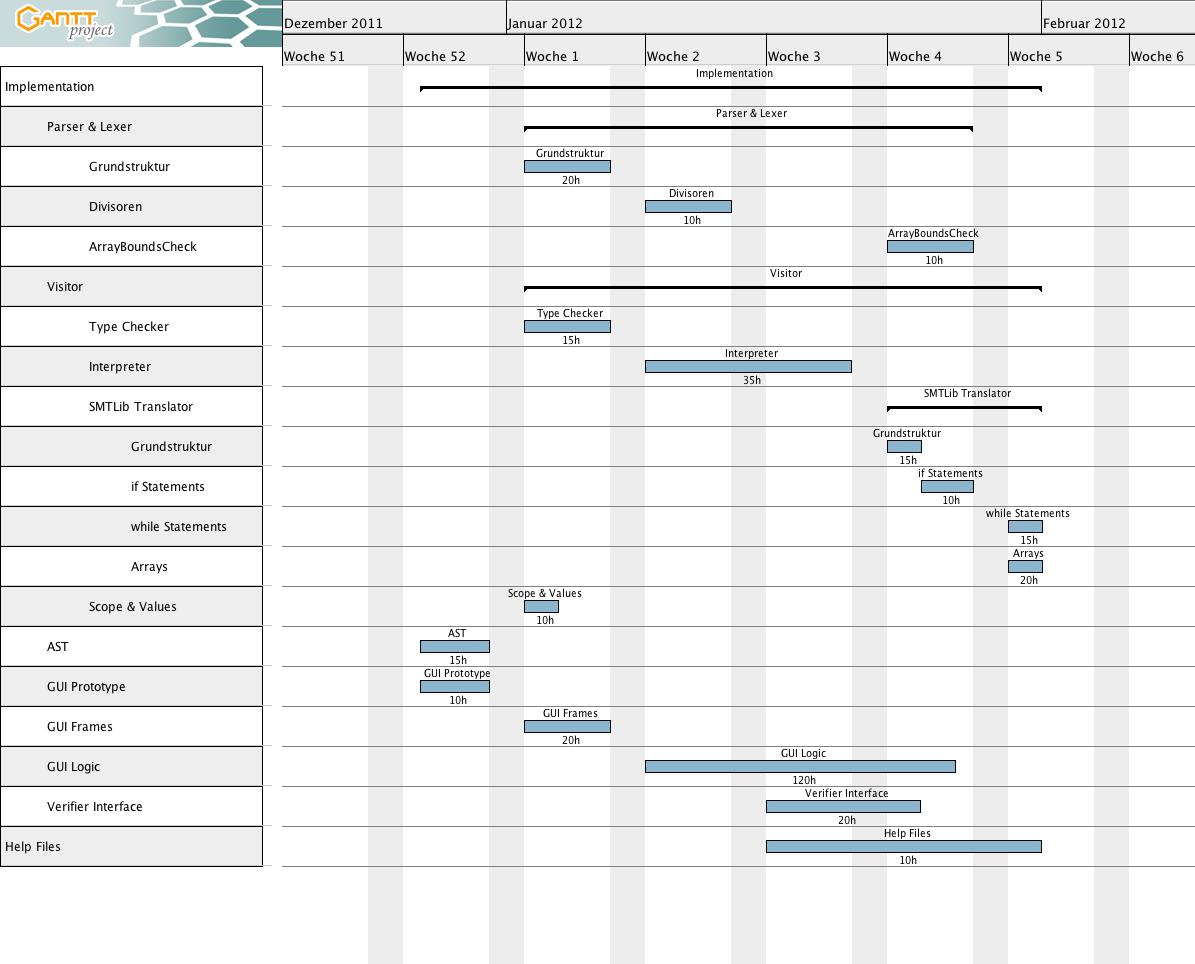
\includegraphics[width=\textwidth]{ImplementierungszeitplanReal.png}
\end{landscape}

\subsection{Parser und Lexer}
Die Implementierung von Parser und Lexer dauerte - insbesondere aufgrund von Sonderf\"{a}llen wie der Division durch Null und dem Pr\"{u}fen von Arraygrenzen - l\"{a}nger als urspr\"{u}nglich geplant.
\subsection{Visitor-Klassen}
Der Type Checker nahm weniger Zeit in Anspruch, als daf\"{u}r veranschlagt war. So konnte parallel dazu schon mit der Implementierung der Scope- und Value-Klassen begonnen werden.\\
Die Fertigstellung des Interpreters verz\"{o}gerte sich um etwa eine Woche, da hier Abh\"{a}ngigkeiten vom Interpreter bestanden.\\
Da die Designentscheidungen f\"{u}r die Beweiserschnittstelle \"{u}berarbeitet wurden, fing dessen tats\"{a}chliche Implementierung sp\"{a}ter an als geplant. Durch die Verschiebungen bei Interpreter und Parser kam es ebenfalls zu einem Aufschub bei der Anbindung an den Beweiser mittles des SMTLib Translators.\\
\subsection{GUI}
Die Zeit, die f\"{u}r die Erstellung der GUI ben\"{o}tigt wurde, ist aufgrund von \"{A}nderungen des Klassenentwurfs h\"{o}her ausgefallen, als urspr\"{u}nglich gesch\"{a}tzt wurde.
Durch die \"{A}nderungen des Entwurfs der GUI, die in der Implementierungsphase stattfanden, wurde diese weiter von anderen Komponenten entkoppelt, wodurch die GUI und die AST- bzw. Visitor-Komponenten gr\"{o}\ss tenteils unabh\"{a}ngig voneinander entwickelt werden konnten. Hierdurch entstand im Zeitplan eine gr\"{o}\ss ere Flexibilit\"{a}t.
\subsection{Buffer und Integration}
Die Zeit f\"{u}r Buffer und Integration wurde haupts\"{a}chlich zur weiteren Implementierung verwendet. Die Integration fand zu gro\ss en Teilen w\"{a}hrend der Zeit der Implementierung der GUI Logic statt.